\section{Results}\label{sec:results}
\subsection{Nominal tracking and tuning}
\Cref{tab:nominal} and \cref{fig:nominal,fig:tuning} show the original and retuned comparisons. Original LQI has the lowest nominal IAE (7304.8~$^\circ$C s), but equal-budget tuning changes the nominal training-scenario comparison to LQR (7180.2), LQI (7236.8), and PID (7455.0). This is a conditional ranking under the declared objective, not evidence of universal superiority.
\begin{table}[!htbp]\centering\caption{Original and retuned nominal comparison generated by Rust.}\label{tab:nominal}\resizebox{\linewidth}{!}{\begin{tabular}{llrrr}\toprule
Design & Controller & IAE ($^\circ$C s) & RMSE ($^\circ$C) & Settling (s) \\
\midrule
Original & PID & 7584.2 & 6.227 & 600 \\
Original & LQR & 8068.3 & 6.272 & 837 \\
Original & LQI & 7304.8 & 6.208 & 517 \\
Retuned & PID & 7455.0 & 6.221 & 605 \\
Retuned & LQR & 7180.2 & 6.207 & 502 \\
Retuned & LQI & 7236.8 & 6.207 & 508 \\
\bottomrule\end{tabular}
}\end{table}
\begin{figure}[!htbp]\centering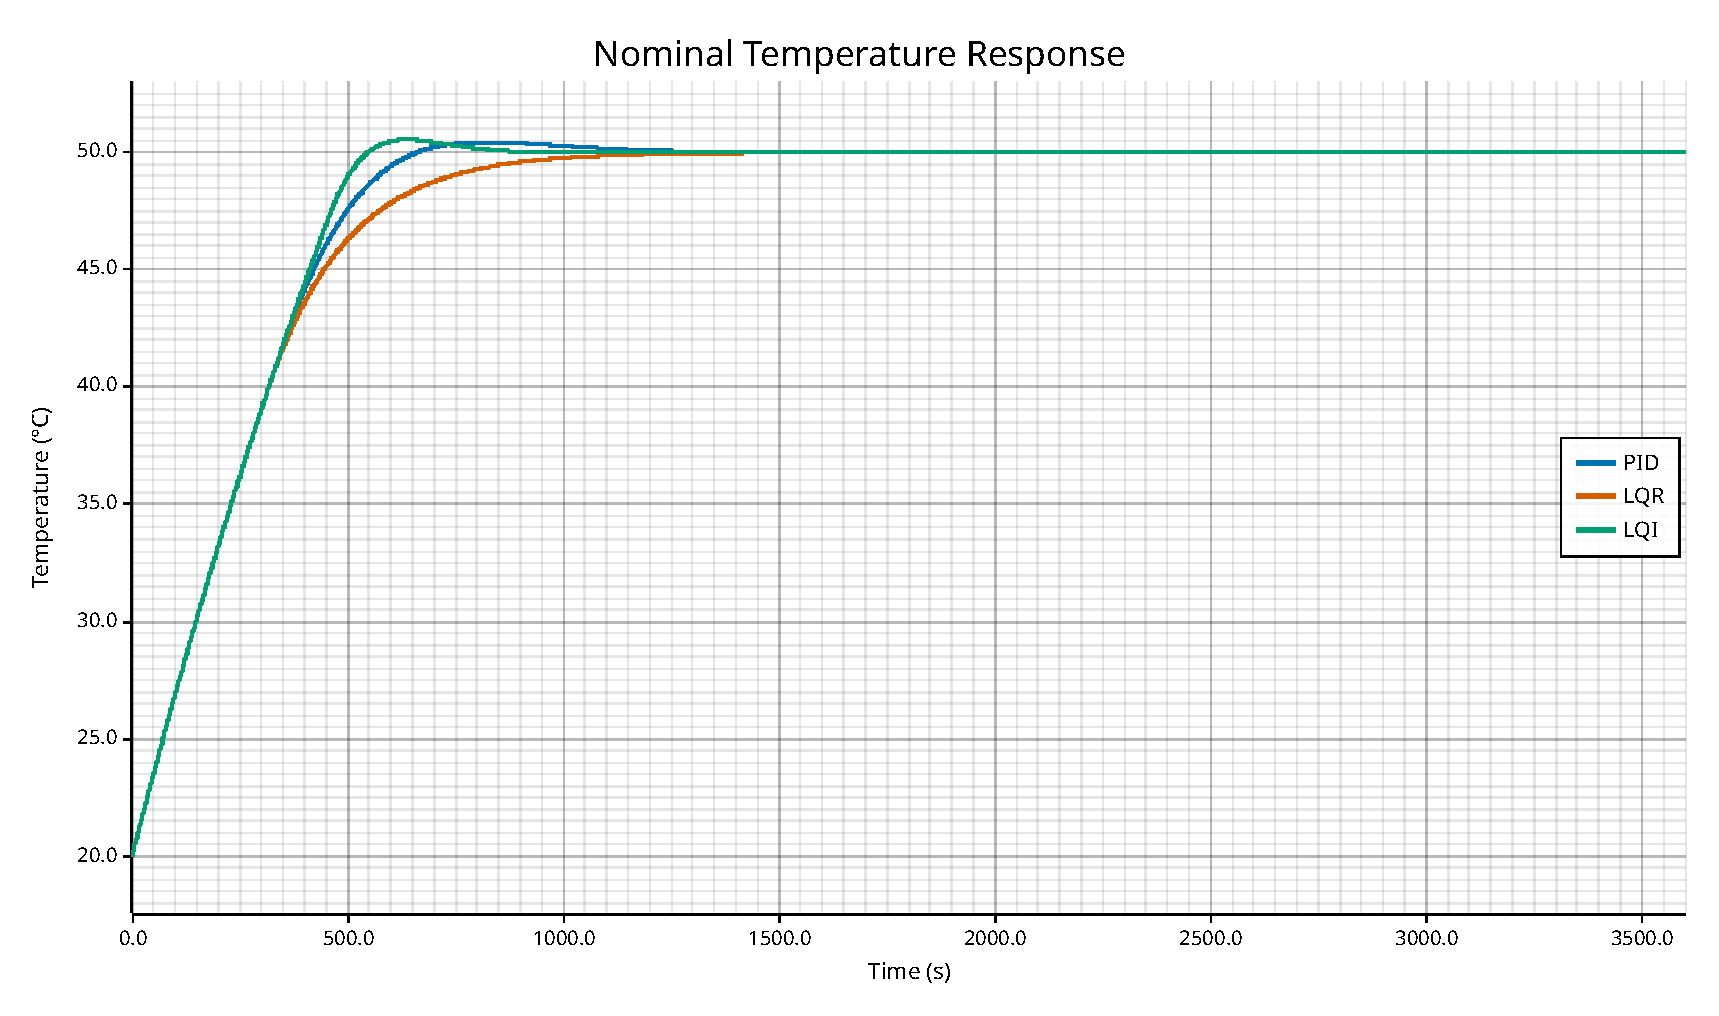
\includegraphics[width=\linewidth]{figures/nominal-temperature.pdf}\caption{Original-controller nominal tracking.}\label{fig:nominal}\end{figure}
\begin{figure}[!htbp]\centering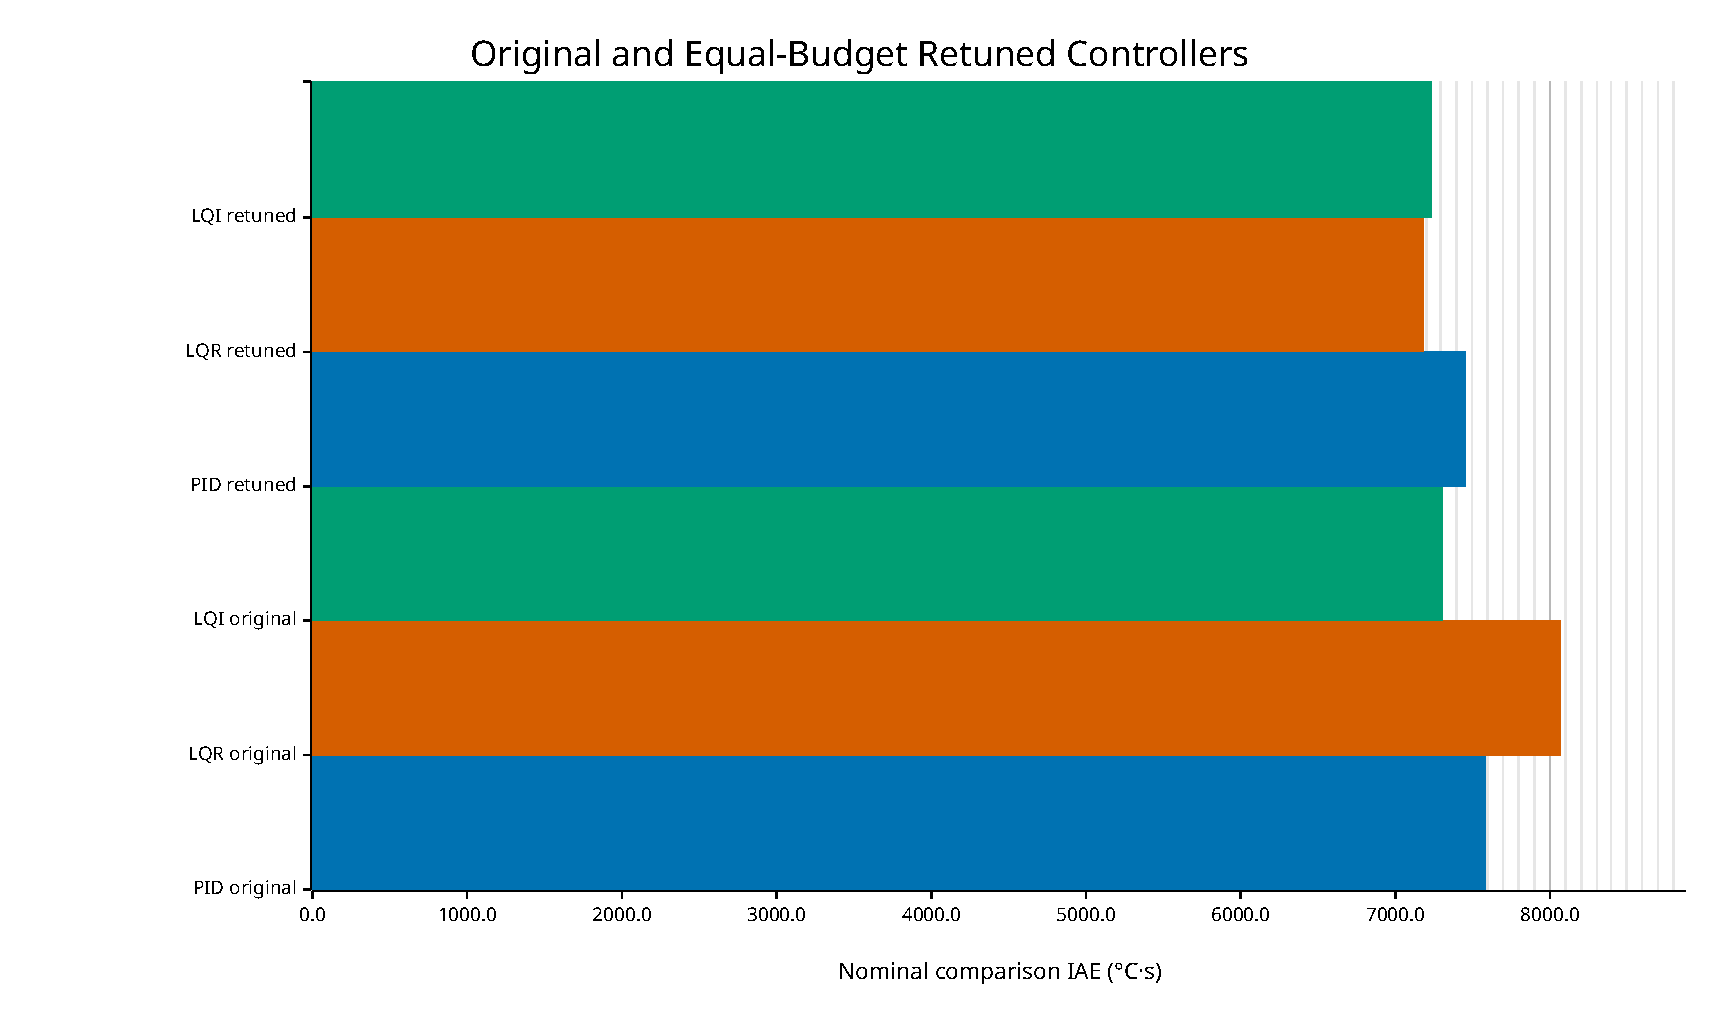
\includegraphics[width=\linewidth]{figures/original-vs-retuned.pdf}\caption{Original versus equal-budget retuned nominal IAE.}\label{fig:tuning}\end{figure}

\subsection{Uncertainty and constant-load rejection}
Capacity uncertainty changes original-controller RMSE ranges by 1.824, 1.898, and \SI{1.878}{\celsius} for PID, LQR, and LQI; equal-percentage $UA$ variation changes them by only 0.196, 0.276, and \SI{0.203}{\celsius}. Capacity therefore dominates this fixed-horizon metric within the tested domain (\cref{fig:uncertainty}).
\begin{figure*}[!t]\centering
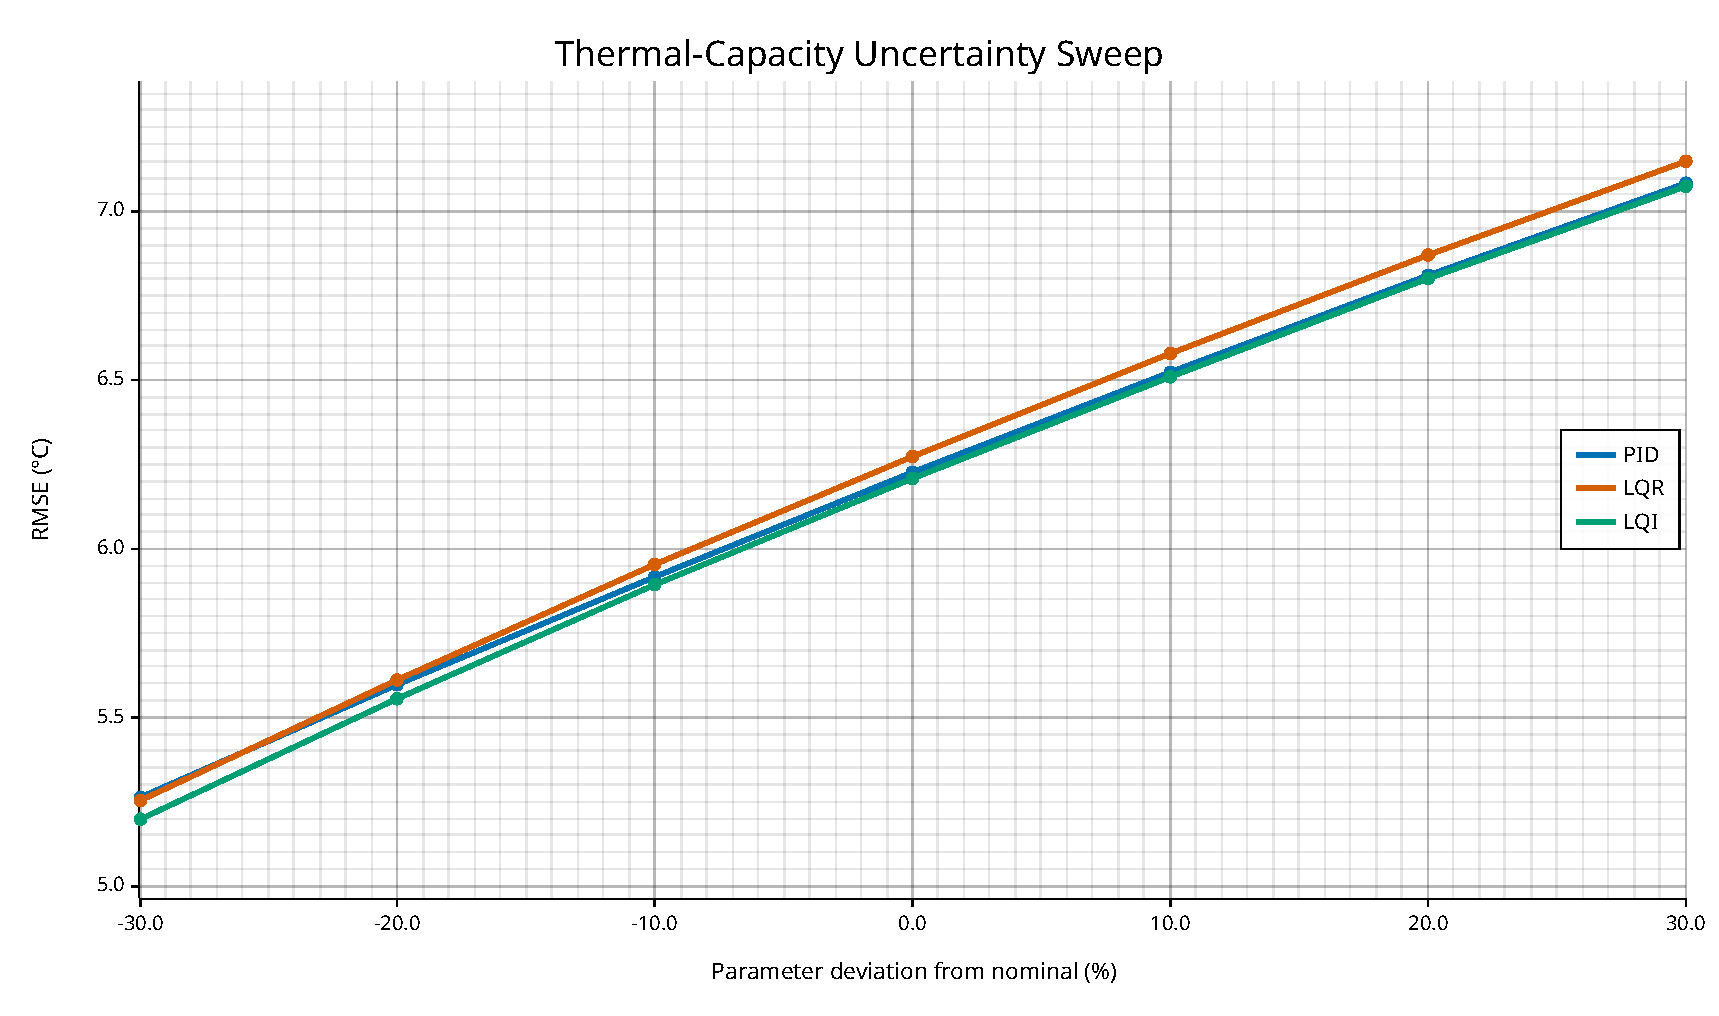
\includegraphics[width=.49\textwidth]{figures/capacity-uncertainty.pdf}\hfill
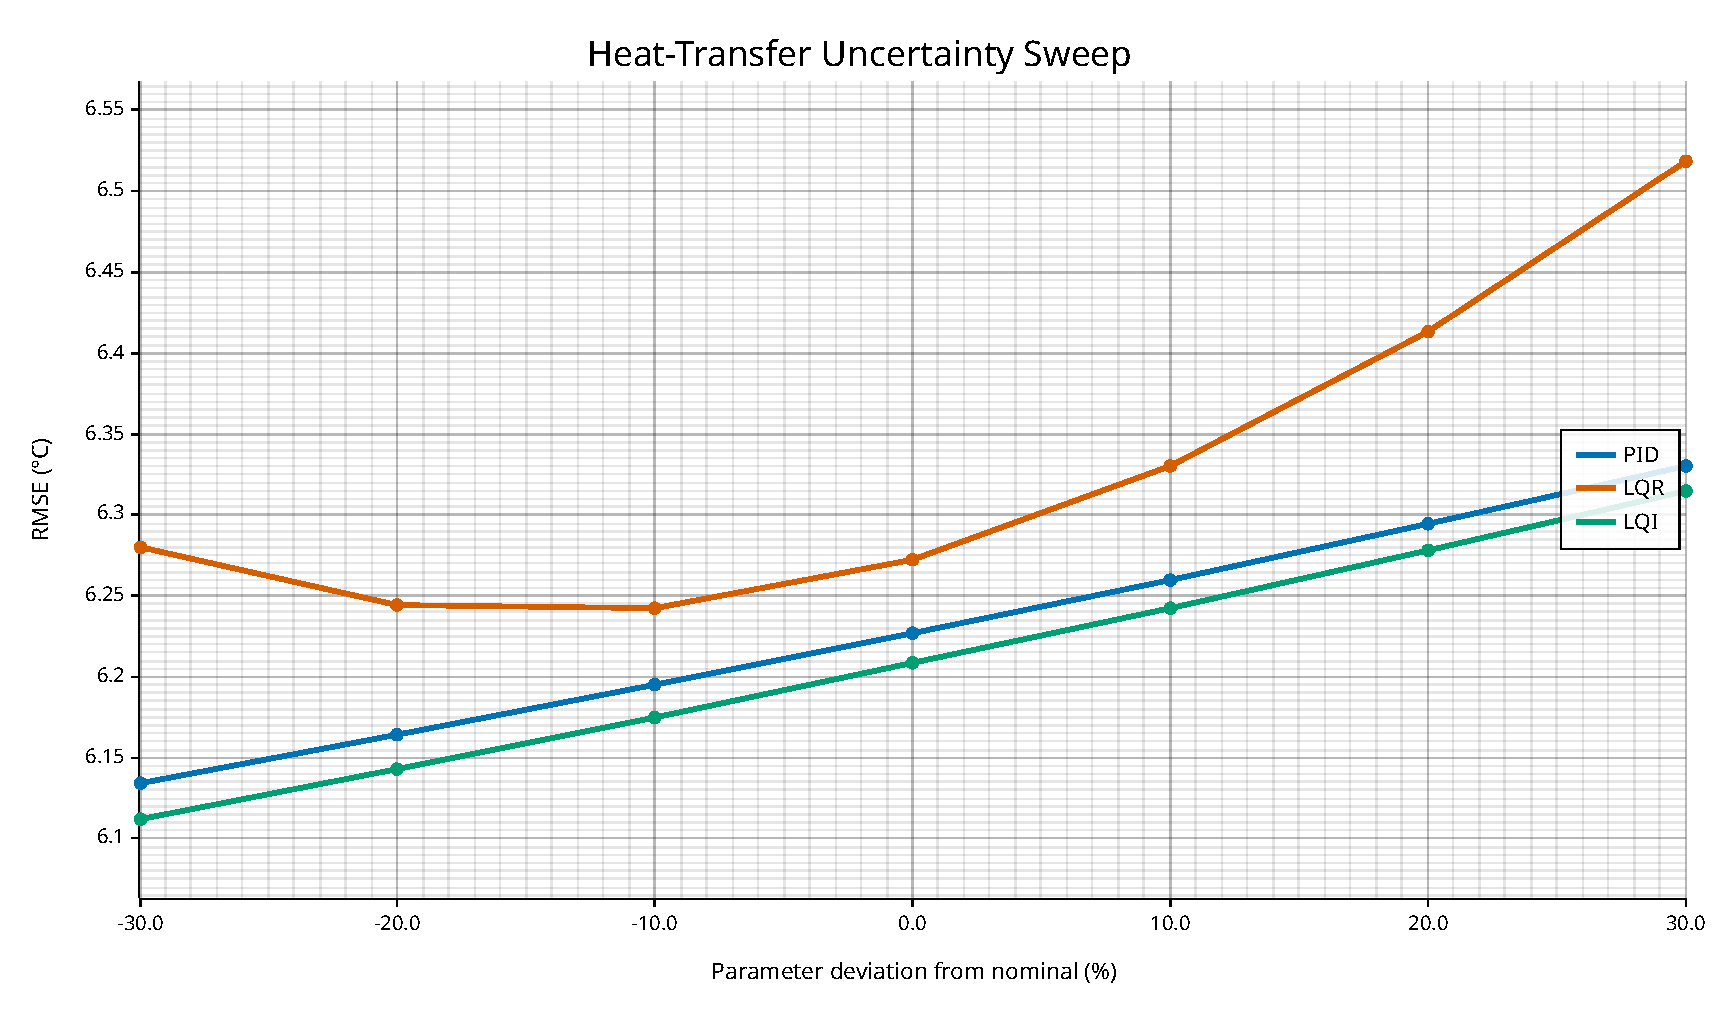
\includegraphics[width=.49\textwidth]{figures/heat-transfer-uncertainty.pdf}
\caption{RMSE sensitivity to isolated thermal-capacity (left) and heat-transfer (right) uncertainty.}\label{fig:uncertainty}\end{figure*}

After the $-\SI{700}{W}$ test load, original-controller post-step IAE is 365.1 (PID), 5006.4 (LQR), and 118.9~$^\circ$C s (LQI). Tail errors are approximately 0, 3.099, and \SI{0}{\celsius}, respectively. Retuned LQR reduces its tail error to \SI{0.079}{\celsius} through much stronger proportional feedback but still lacks structural integral rejection.
\begin{figure}[!htbp]\centering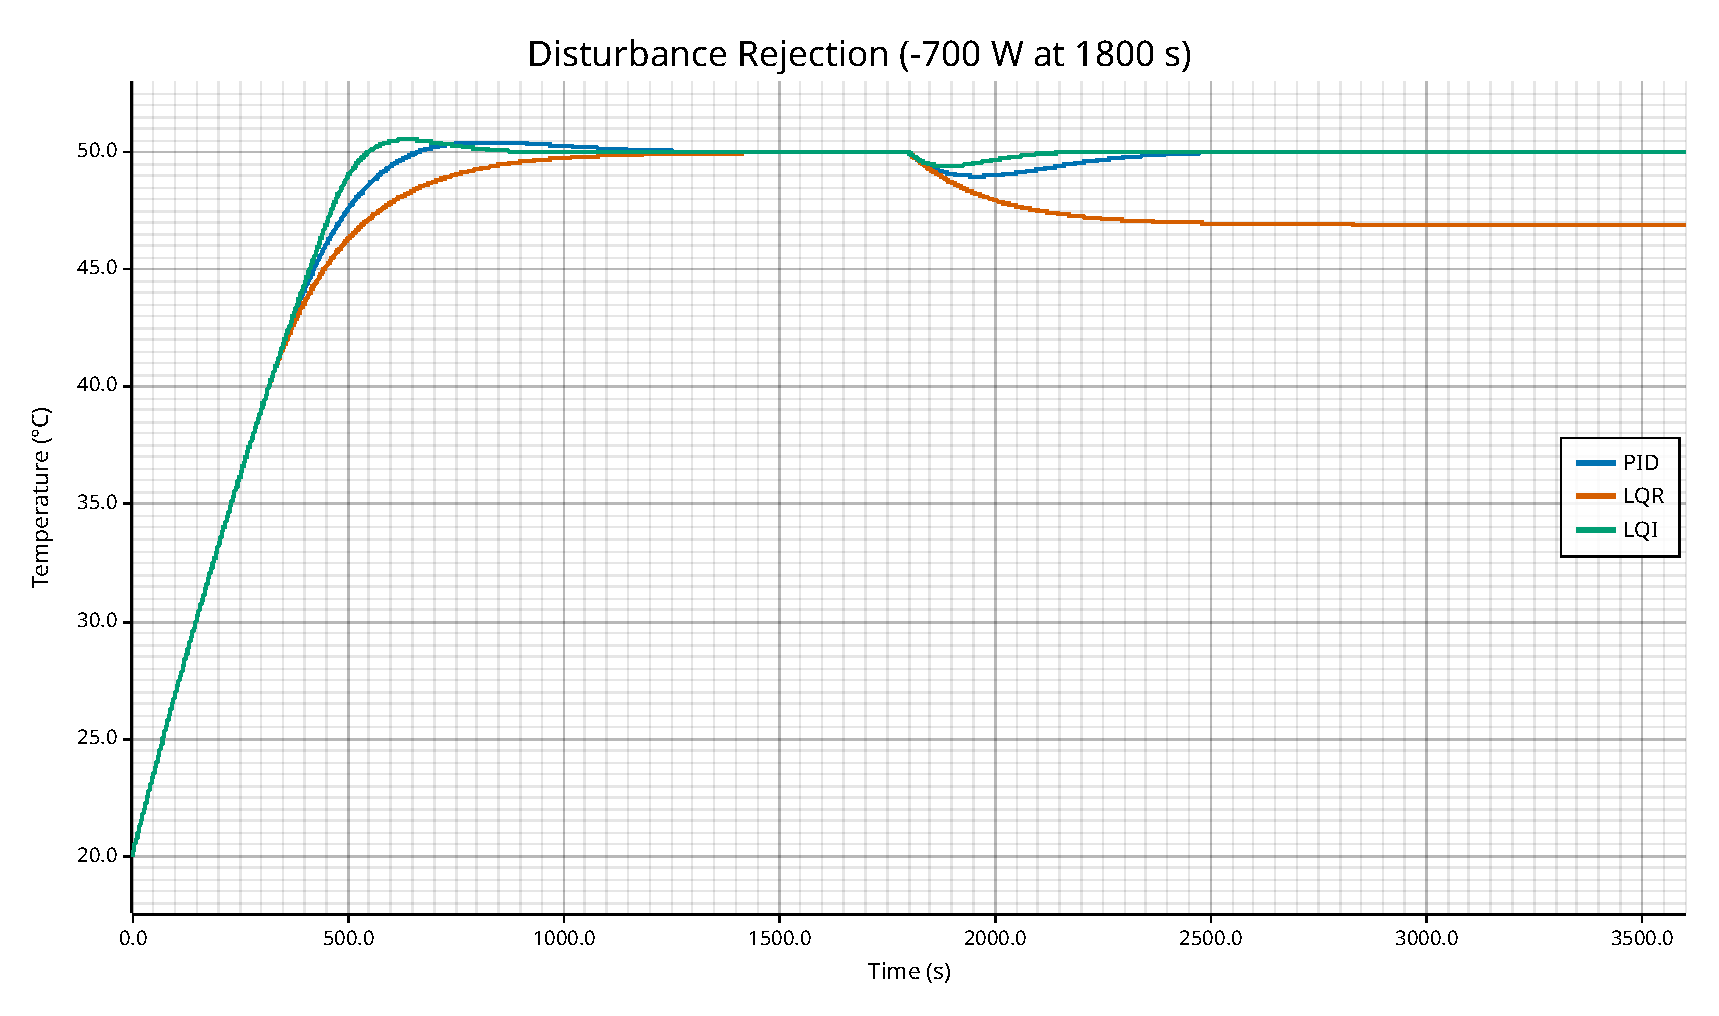
\includegraphics[width=\linewidth]{figures/disturbance-rejection.pdf}\caption{Original-controller response to a $-\SI{700}{W}$ load at \SI{1800}{s}.}\label{fig:disturbance}\end{figure}

\subsection{Saturation and noise}
Corrected original restricted-actuator IAE is 25231.4 (PID), 25268.5 (LQR), and 25209.8~$^\circ$C s (LQI); the original pre-audit claim that LQR won was caused by incorrect anti-windup limits. Retuned restricted-actuator ranking is LQR (25200.3), LQI (25204.6), PID (25221.5), a small ranking change relative to retuned nominal results. Differences are tiny relative to the common saturation-dominated transient.
\begin{figure}[t]\centering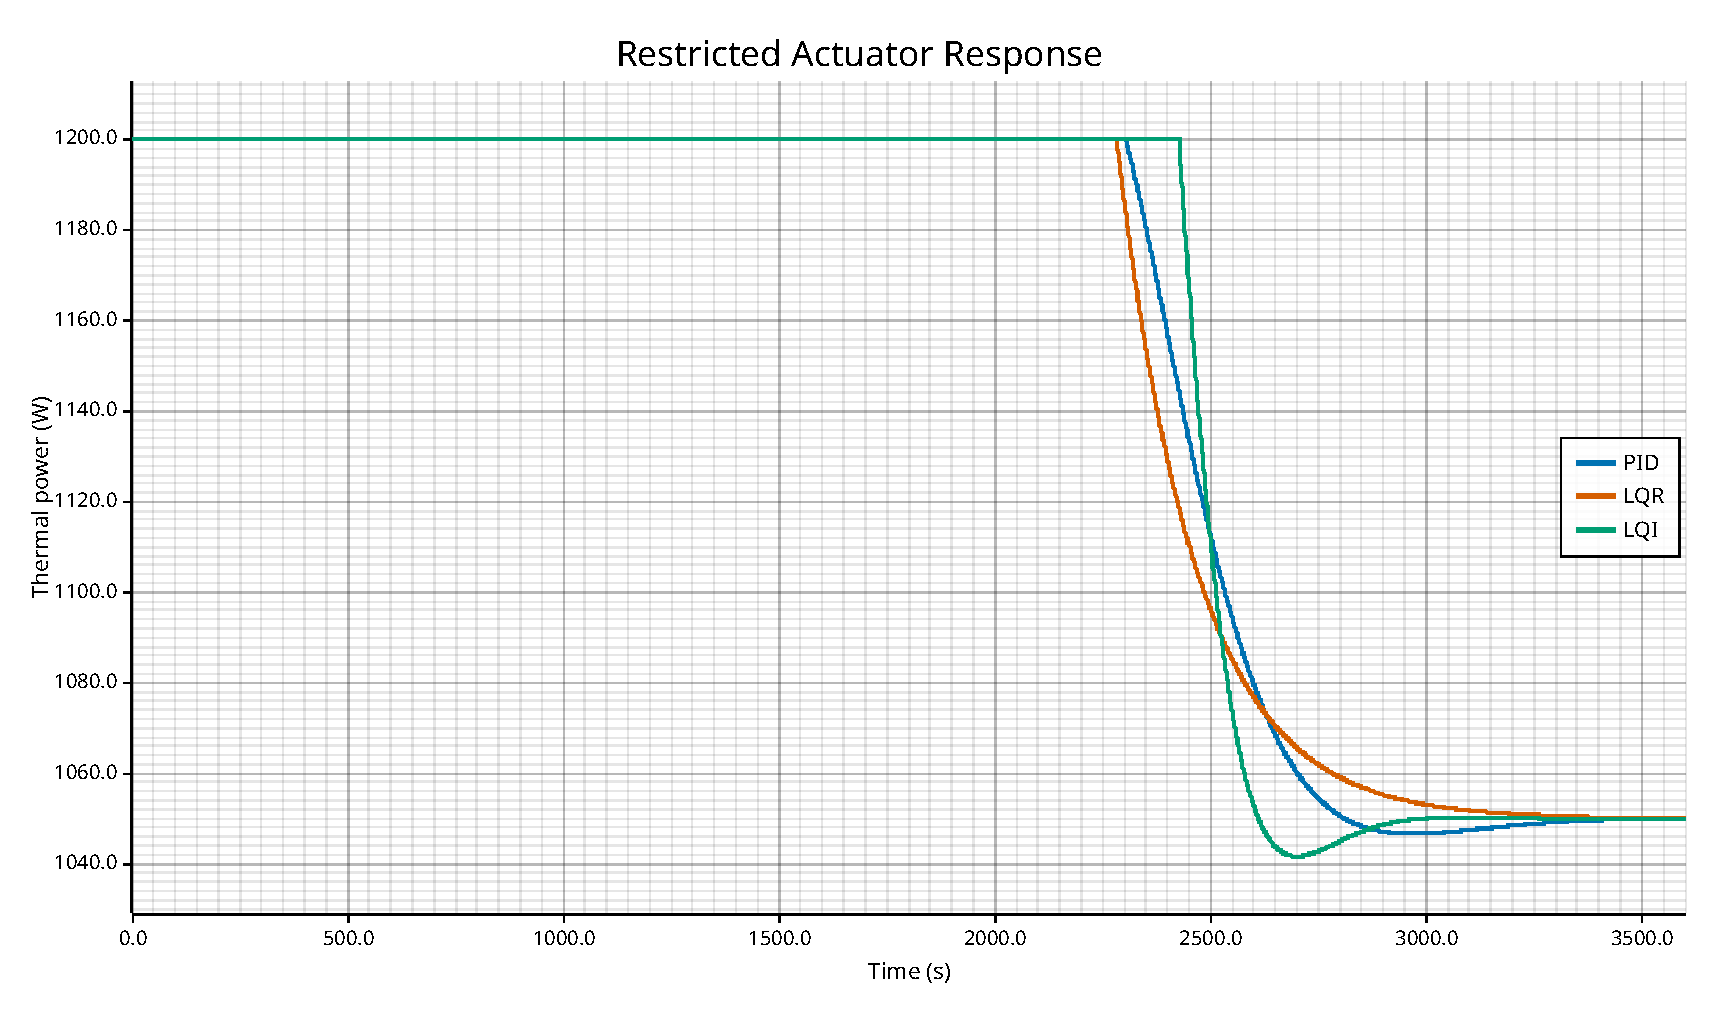
\includegraphics[width=\linewidth]{figures/actuator-saturation.pdf}\caption{Applied power under restricted limits for original controllers.}\label{fig:saturation}\end{figure}

Steady-regime paired LQI-minus-PID noise RMSE is \SI{0.004216}{\celsius} (95\% CI 0.003978--0.004453, $d_z=3.52$). Although standardized against very small replicate variability, four thousandths of a degree is practically negligible for the idealized process. Changing noise magnitude or spectrum may change this conclusion; no broad sensor claim is made.
\begin{figure}[t]\centering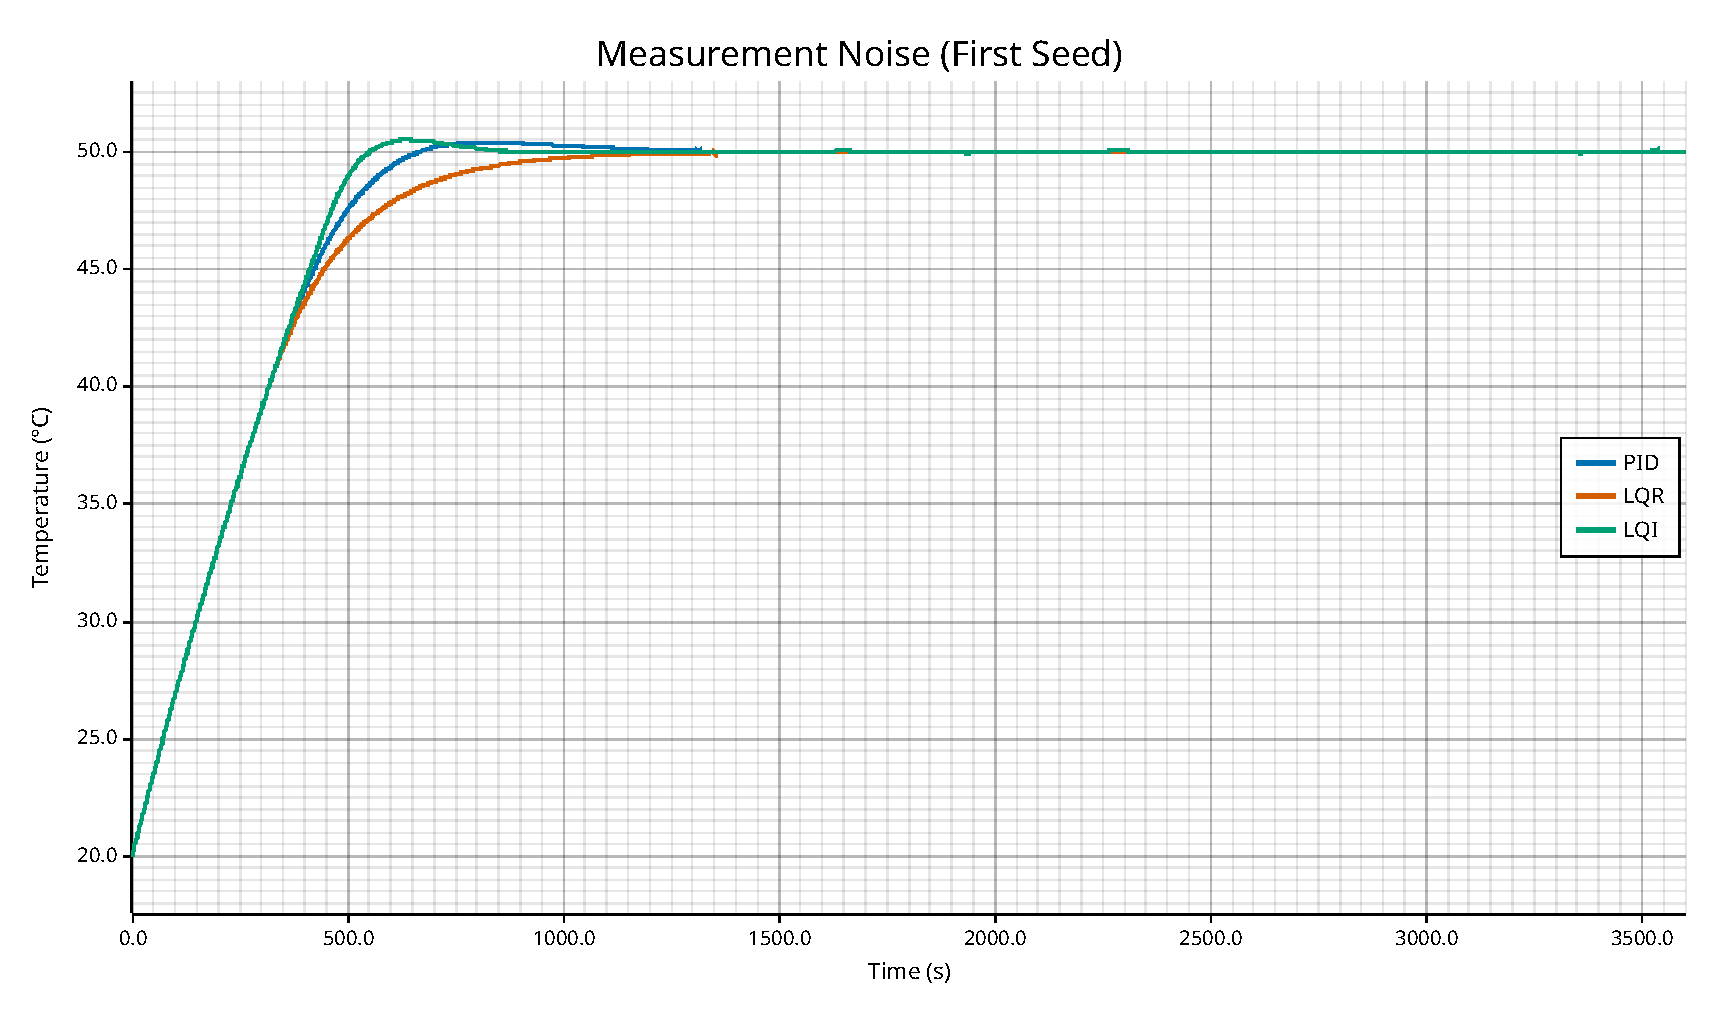
\includegraphics[width=\linewidth]{figures/measurement-noise.pdf}\caption{One paired realization with \SI{0.15}{\celsius} measurement noise.}\label{fig:noise}\end{figure}

\subsection{Unmodeled sensor dynamics}
The lag-and-delay plant exposes a retuning trade-off (\cref{tab:fidelity,fig:fidelity}). Retuned LQR IAE rises to 9345.2~$^\circ$C s, does not settle, and saturates for 2739~s, whereas original LQR IAE is 7804.1. PID and LQI change much less. Aggressive nominal tuning therefore improves the simple plant while reducing tolerance to omitted sensing dynamics.
\begin{table}[!htbp]\centering\caption{Sensor-lag and delay results generated by Rust.}\label{tab:fidelity}\resizebox{\linewidth}{!}{\begin{tabular}{llrrr}\toprule
Design & Controller & IAE ($^\circ$C s) & RMSE ($^\circ$C) & Saturation (s) \\
\midrule
Original & PID & 7447.1 & 6.218 & 365 \\
Original & LQR & 7804.1 & 6.245 & 344 \\
Original & LQI & 7289.2 & 6.208 & 488 \\
Retuned & PID & 7364.1 & 6.215 & 395 \\
Retuned & LQR & 9345.2 & 6.252 & 2739 \\
Retuned & LQI & 7295.1 & 6.208 & 507 \\
\bottomrule\end{tabular}
}\end{table}
\begin{figure}[t]\centering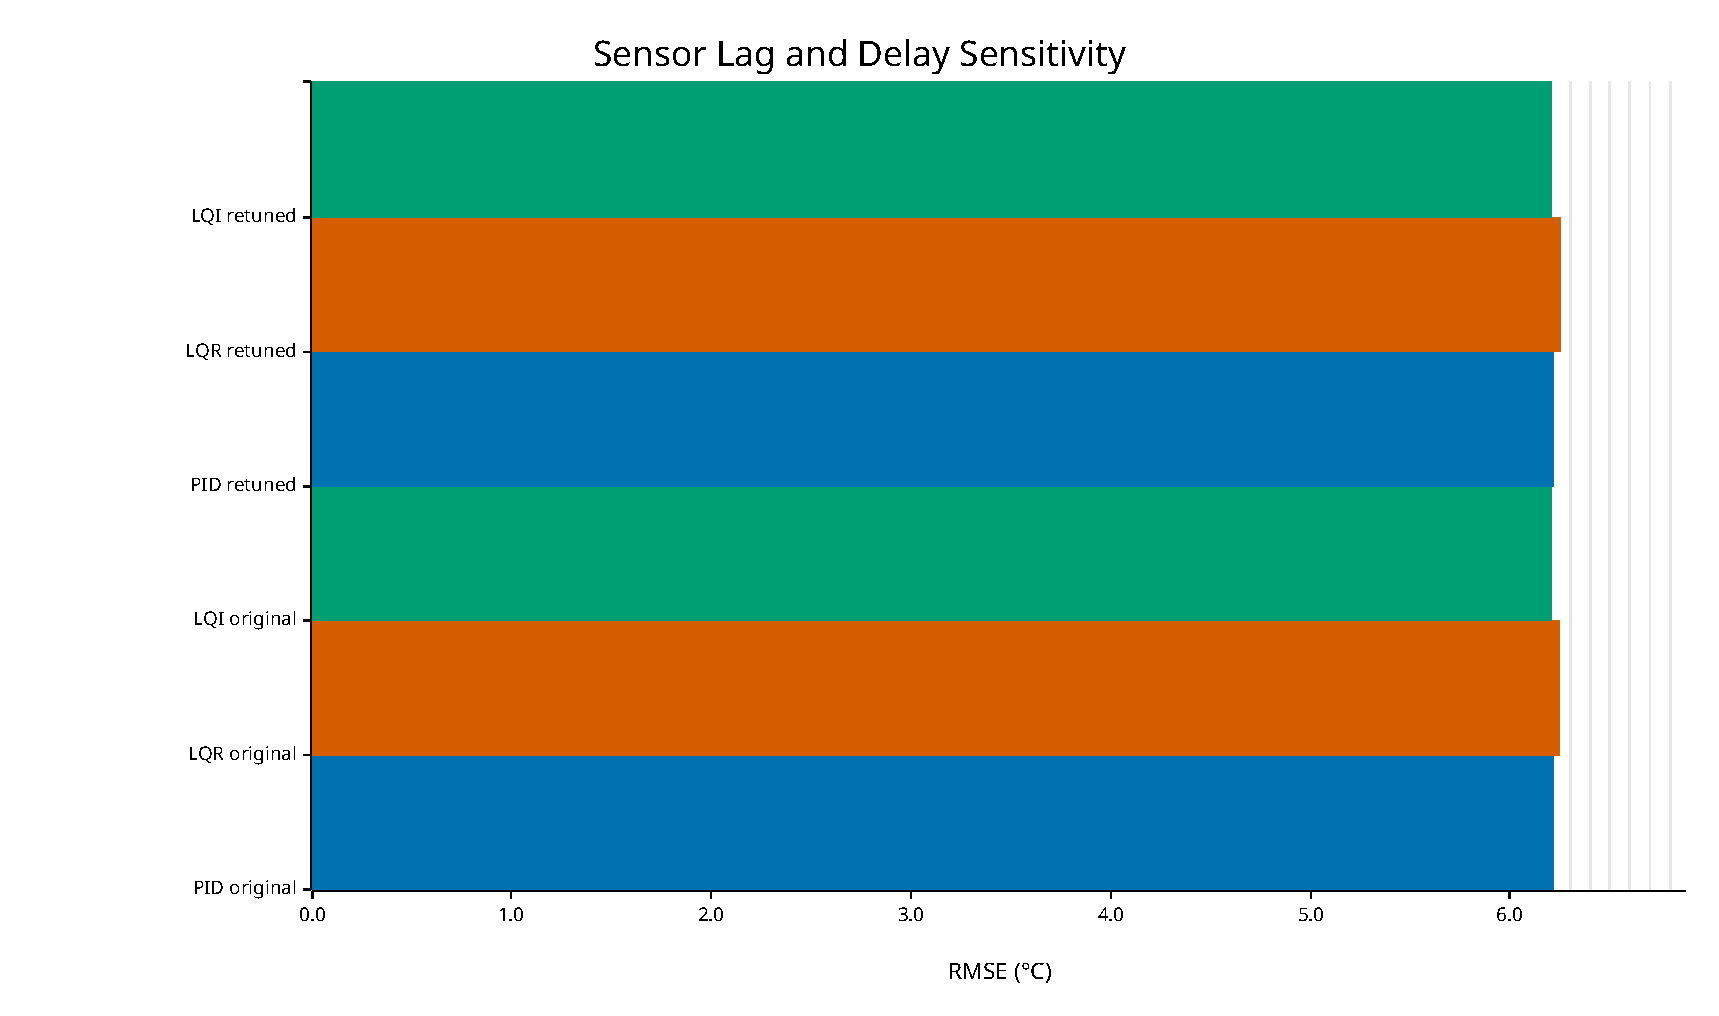
\includegraphics[width=\linewidth]{figures/higher-fidelity-summary.pdf}\caption{RMSE with a \SI{20}{s} sensor lag and \SI{10}{s} delay.}\label{fig:fidelity}\end{figure}
\FloatBarrier

